% !TeX encoding = UTF-8
% !TeX program = xelatex
% !TeX spellcheck = en_US

\documentclass[degree=bachelor]{ustcthesis}
% degree      = doctor | master | bachelor
% degree-type = academic | professional | engineering
% language    = chinese | english
% fontset     = windows | mac | ubuntu | fandol

% 加载宏包、全部的配置
\input{ustcsetup}


\begin{document}


\ustcsetup{
    title={基于生成式先验的人像视频编辑},
    title*={Portrait Video Editing Based on Generative Prior},
    author={汪兆辰},
    student-id={PB21010362},
    speciality={信息与计算科学},
    supervisor={张举勇}
}
\maketitle
% \copyrightpage

\frontmatter
% \include{chapters/innovations}  % 博士学位论文的创新性说明
% !TeX root = ../main.tex

\ustcsetup{
  keywords  = {学位论文, 摘要, 关键词},
  keywords* = {Dissertation, Abstract, Keywords},
}

\begin{abstract}
  随着数字媒体技术的飞速发展和短视频平台的普及,视频内容创作已成为互联网时代的重要表达方式。
  其中,肖像视频编辑作为视频处理领域的核心应用之一,在影视制作、社交媒体、虚拟现实等领域具有广泛需求。
  传统的生成式人工智能视频编辑方法主要依赖于2D图像处理技术,难以满足3D场景下的高质量、高效率编辑需求。

  在这一背景下,PortraitGen系统代表了当前肖像视频编辑技术的前沿水平。该系统通过将2D肖像视频编辑问题
  提升至3D领域,利用动态3D高斯场确保空间和时间一致性,并创新性地引入神经高斯纹理机制,实现了高质量、
  高效率的多模态肖像视频编辑。
  
  本文基于PortraitGen算法设计并实现了一个完整的视频编辑系统,采用前后端分离的系统架构,开发了完整的
  用户工作流,并实现了管理员监控系统,以支持用户的行为分析和数据监控。

\end{abstract}

\begin{abstract*}
  With the rapid development of digital media technology and the widespread adoption of short 
  video platforms, video content creation has become an essential mode of expression in the 
  internet era. Among these, portrait video editing, as one of the core applications in video 
  processing, holds extensive demand in fields such as film production, social media, and virtual 
  reality. Traditional AIGC video editing methods primarily rely on 2D image 
  processing techniques, making it difficult to meet the requirements for high-quality and 
  high-efficiency editing in 3D scenarios.

  Against this backdrop, the PortraitGen system represents the cutting edge of current portrait 
  video editing technology. By elevating the 2D portrait video editing problem into the 3D domain, 
  the system employs a dynamic 3D Gaussian field to ensure spatial and temporal consistency while 
  innovatively introducing a Neural Gaussian Texture mechanism, thereby achieving high-quality, 
  efficient, and multimodal portrait video editing.

  This paper designs and implements a comprehensive video editing system based on the PortraitGen 
  algorithm. Adopting a frontend-backend decoupled architecture, the system develops a complete 
  user workflow and implements an administrator monitoring system to support user behavior 
  analysis and data monitoring.
\end{abstract*}

\tableofcontents
% \listoffigures
% \listoftables
\listoffiguresandtables
% \include{chapters/notation}

\mainmatter
% !TeX root = ../main.tex

\chapter{引言}

\section{研究背景与意义}

\subsection{研究背景}

随着人工智能技术的快速发展和5G网络的全面普及,全球数字内容产业正在经历前所未有的变革。
根据国家广电总局最新发布的《中国网络视听发展研究报告(2025)》显示,中国网络视听用户规模
已达10.91亿,其中短视频用户规模突破10.40亿,日均使用时长高达156分钟,稳居各类互联网应用之首。
这一庞大的用户基数和旺盛的内容创作需求,对视频编辑技术提出了更高要求,特别是在实时性、
智能化和个性化方面。

当前,AI视频编辑技术已成为行业关注的焦点。以PortraitGen为代表的先进算法已能实现100FPS的高效渲染,
支持文本、图像驱动的多模态编辑;Live2Diff采用单向的时间注意力机制,能够以近乎实时的速度将实时视频流
转换为风格化内容;ChatAnyone等风格化肖像视频生成模型的发展也十分迅速。然而,这些前沿算法在实际应用
中仍面临着诸多挑战,由于缺乏完善的用户交互
设计,限制了其广泛推广和应用,提高了前沿技术的使用门槛;另外,因为没有直接面向用户,研究者往往无法了解
用户的真实需求与体验反馈。

\subsection{研究意义}

本研究基于PortraitGen算法,构建了一套完整的智能视频编辑系统。我们设计了直观的用户界面与用户工作流,使
用户无需关心算法细节,即可轻松实现视频在文字、图像等多模态输入下的风格化处理、虚拟合成、背景光重构等功能。
同时,我们搭建了管理员系统,使研究者可以通过用户反馈和操作日志,了解用户的使用情况,从而根据用户的真实需求
优化算法,调整研究方向。

本文的主要贡献包括:
\begin{itemize}
    \item 提出面向生产环境的PortraitGen工程化方案,实现算法到产品的完整转化
    \item 设计了可扩展的用户工作流,可以搭载多种算法,实现各种算法的切换
    \item 通过实际应用验证,为行业提供可复制的技术方案
\end{itemize}

\section{论文结构}

本文的组织结构如下:
\begin{itemize}
    \item \textbf{引言}:介绍研究的背景与意义
    \item \textbf{相关工作}:详细讨论PortraitGen技术原理、现有视频编辑App的现状以及技术栈选择;
    \item \textbf{系统设计}:介绍系统的整体架构、前端设计、后端设计、数据库设计及安全性设计;
    \item \textbf{功能实现}:详细描述用户管理、视频编辑功能及管理员功能的实现细节;
    \item \textbf{性能评估}:通过功能测试、性能测试及用户体验评估,验证系统的有效性和稳定性;
    \item \textbf{改进与展望}:提出系统改进方向和未来工作展望;
    \item \textbf{结论}:总结本文的研究成果,强调本文的贡献及未来展望。
\end{itemize}


\chapter{相关技术与工作}

\section{传统视频编辑方法}

早期的肖像视频编辑主要依赖于生成对抗网络(GAN),StyleGAN2在图像生成方面取得成功后,许多工作者
开始将预训练的GAN模型应用于肖像编辑,例如3D-FM GAN引入StyleGAN以在保留人脸特征的同时实现3D人脸编辑;
此外,也有工作将其应用于肖像的风格化,DualStyleGAN针对当时即便使用大量同类训练数据也只能实现单一风格化的问题,
引入StyleGAN实现了利用一张模板的风格化肖像生成。但是由于StyleGAN2的表示能力有限,这些工作难以稳定地
在复杂场景下实现高质量的肖像生成。

为了寻求更强的表示能力,研究者们尝试使用3D表示来进行肖像编辑。ClipFace引入了三维网格来表示人脸,用自监督的生成模型
来实现人脸的编辑与动画。然而受限于三维网格的表示能力,这些工作存在身份失真与动作失真等问题。NeRF在三维重建方面
取得巨大突破后,许多工作也引入NeRF进行肖像编辑,但这些工作仍然不能满足许多应用的需要。

扩散模型被提出并获得巨大成功后,许多工作尝试利用扩散模型强大的生成能力。Arc2Face、Next3d等工作在2D肖像图片的生成与
编辑方面取得了进展;在3D方面,扩散模型被应用于文字提示下的3D人脸生成,而Avatarstudio和Control4D则尝试将扩散模型应用于3D人脸编辑,
但它们都需要多角度的动态视频序列作为输入来建模3D人脸,这在现实中比较难以获取。

\section{PortraitGen技术原理}

PortraitGen作为当前先进的肖像视频编辑技术,其核心创新点体现在以下三个关键方面。

\subsection{3D高斯场表示}

\subsubsection{3D高斯场景表示}
在PortraitGen中,我们将视频编辑任务从2D提升至3D,并采用3D高斯溅射来表示场景。具体而言,
我们用数百万个3D高斯椭球来表示场景,对于每个以$\symbf{x}_0$为球心的高斯分布,我们有
\begin{equation}
    g(\symbf{x})=\exp{-\frac{1}{2}(\symbf{x}-\symbf{x}_0)^T\symbf{\Sigma}(\symbf{x}-\symbf{x}_0)}
\end{equation}
其中$\symbf{\Sigma}$为协方差矩阵,通过旋转和缩放控制椭球的形状,有分解
\begin{equation}
    \symbf{\Sigma}=\symbf{R}\symbf{\Lambda}\symbf{\Lambda}^T\symbf{R}^T
    \label{cov-decom}
\end{equation}
其中$\symbf{R}$为旋转矩阵,$\symbf{\Lambda}$为缩放矩阵。为了将三维的场景映射到二维平面,
我们还需要定义每个3D高斯的不透明度$\alpha$和球谐函数,以控制光照和颜色信息。

\subsubsection{参数优化}
3D高斯场采用了可微分的溅射渲染,通过将3D高斯投影到2D屏幕空间,我们可以计算每个像素的颜色
\begin{equation}
    C(\symbf{p})=\sum_{i\in N}c_i\alpha_i\prod_{j=1}^{i-1}(1-\alpha_j)
\end{equation}
其中$c_i$为第$i$个高斯的颜色,基于视角可以由球谐函数决定。为了优化由稀疏点云重建的3D高斯场,
我们将给定视角下的渲染结果与真实结果进行比对,定义损失函数为
\begin{equation}
    \mathcal{L}=(1-\lambda)\mathcal{L}_1+\lambda\mathcal{L}_\text{D\_SSIM}
\end{equation}
其中$\mathcal{L}_1$为渲染的像素差异,描述了渲染结果与真是结果的光度差异;$\mathcal{L}_\text{D\_SSIM}$
为基于感知的损失函数,用于衡量图像的结构相似性。我们选用随机梯度下降(SGD)来优化3D高斯的参数,
包括高斯的位置、协方差、不透明度和颜色。注意到协方差矩阵$\symbf{\Sigma}$有其物理意义,只有半正定矩阵
是合理的,但是SGD优化难以添加约束条件,因此考虑到协方差矩阵的分解形式~\eqref{cov-decom},我们转而对
代表缩放的向量$\symbf{s}$与代表旋转的四元数$\symbf{q}$进行优化。

初始的3D高斯直接由点云重建,而这种2D到3D的映射往往无法满足精细表示的需要,因此我们的优化也需要
有3D高斯的自适应操作,包括:
\begin{enumerate}
    \item \textbf{删除}:当3D高斯的透明度小于阈值$\epsilon_{\alpha}$时,说明此时3D高斯对场景表示的贡献较小,可以删除;
    \item \textbf{密集}:区域没有被3D高斯覆盖与过度覆盖都说明当前重建不够,需要修改目前的3D高斯,以更好地表示场景:
        \begin{itemize}
            \item 当区域没有被3D高斯完全覆盖时,将已有的3D高斯复制并按照梯度方向移动到空白位置;
            \item 当区域被3D高斯过度覆盖时,将大3D高斯按照$\phi=1.6$的比例分成两个小的3D高斯;
        \end{itemize}
    \item \textbf{特殊处理}:与其他体积表征的方法类似,在相机附近可能有悬浮3D高斯导致优化停滞,因此需要每迭代3000轮后将这些3D高斯的透明度$\alpha$设置为接近0。
\end{enumerate}

\begin{figure}[ht]
    \centering
    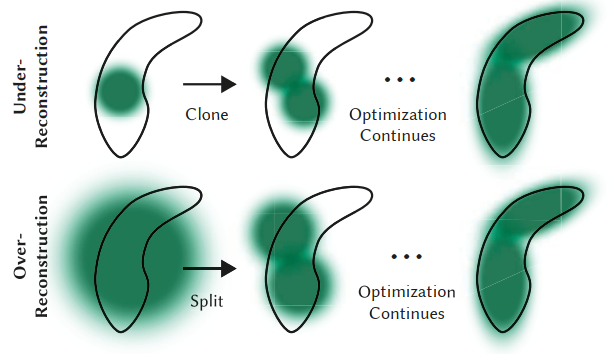
\includegraphics[width=0.5\textwidth]{source/img/gauss_recon.png}
    \bicaption{3D高斯的密集}{Densification of Gaussian}
\end{figure}

\subsubsection{可微光栅化渲染}

3D高斯的光栅化过程主要分为四个步骤:
\begin{enumerate}
    \item \textbf{分块}:将屏幕空间划分为$16\times 16$的小块,对每个小块保留与视锥相交超过99\%的高斯球;
    \item \textbf{排序}:为每个高斯分配一个键,携带视图空间深度与块ID信息,并利用GPU基数排序,为每个块生成一个高斯列表;
    \item \textbf{光栅化}:每个块启动一个线程块,协作加载高斯到共享内存。对每个像素,从前到后遍历列表,累积颜色和$\alpha$值,当像素的$\alpha$值达到饱和(接近1)时,停止处理;
    \item \textbf{反向传播}:在反向传播时,重新遍历排序后的高斯列表,但方向是从后到前。这样可以在计算梯度时恢复中间的$\alpha$值,无需存储中间结果增加内存消耗。
\end{enumerate}

\subsection{神经高斯纹理机制}

在标准的3D高斯溅射中,每个3D高斯的颜色通过球谐函数的系数来表示,而这种表示存在一些问题:一方面,球谐系数仅能建模低频的光照变化,难以表现高频的细节,如笔触、艺术风格等;另一方面,
强制使所有视角严格遵守物理光照,阻碍了3D高斯在会真实感渲染方面的应用,例如卡通风格的轮廓线等。PortraitGen用可学习的特征来代替每个3D高斯的球谐函数,实现了更强的表达能力。

我们使用SMPL-X作为人体模型的表示方法,SMPL-X的定义为
\begin{align}
    M(\beta,\theta,\psi)&=W(T_p(\beta,\theta,\psi), J(\beta),\theta, \mathcal{W})\\
    T_p(\beta,\theta,\psi)&=\bar{T}+B_S(\beta;\mathcal{S})+B_E(\psi;\mathcal{E})+B_P(\theta;\mathcal{P})
\end{align}
其中$\beta$、$\theta$、$\psi$分别为形状、姿态与表情参数;$W$为线性混合蒙皮函数,$J$为稀疏线性回归器,可以从输入网格顶点回归出三维关节位置,$\mathcal{W}$
为混合权重,在旋转时起平滑作用。

我们在SMPL-X模型的UV表面绑定3D高斯场$\phi$,通过纹理坐标$(u,v)$来索引特征,这样在网格动态变形时高斯能随之运动从而保持拓扑的一致性。利用UV空间的参数映射$\mathcal{G}$,我们可以得到某一帧的3D高斯场
\begin{equation}
    (\symbf{X}_0,Q,S,O,F)=\mathcal{F}(M(\beta,\theta,\psi),\mathcal{G},\phi)
\end{equation}

\subsection{表情相似性引导与感知编辑}

在PortraitGen的编辑过程中,需要迭代编辑视频数据集,而在反复编辑视频帧的过程中,每次编辑都可能引入微小表情偏差,多次迭代后偏差放大,
导致面部表情和个性化特征会逐渐退化,如笑容僵硬、五官变形等。为了解决这一问题,我们采用3D表情识别模型EMOCA提取表情潜码
\begin{equation}
    z_{\text{exp}}=E_{\text{EMOCA}}(I) \in \mathbb{R} ^{50}
\end{equation}
并通过$L2$损失约束编辑后的表情特征
\begin{equation}
    \mathcal{L}_{\text{exp}}=||E_{\text{EMOCA}}(I_{\text{edit}})-E_{\text{EMOCA}}(I_{\text{src}})||_2^2
\end{equation}
实现了仅约束表情肌肉运动而不限制外观风格变化。


\chapter{系统设计}

\section{需求分析}



\section{技术栈选择}

\subsection{前端技术}

本系统采用Next.js作为前端框架,主要基于以下考量:
\begin{enumerate}
    \item \textbf{服务器端渲染}:在服务器渲染React组件,以提升用户的首屏加载速度;
    \item \textbf{静态生成}:在构建时生成静态HTML文件,从而提前生成页面,用户访问时即时加载;
    \item \textbf{TypeScript支持}:支持TypeScript,增加类型检查与面向对象。
\end{enumerate}

\subsection{后端技术}

后端采用用python编写的Flask框架,基于以下的开发需求:
\begin{enumerate}
    \item \textbf{轻量级}:作为轻量级Web框架,Flask不强制使用任何特定库,可以根据需求灵活扩展;
    \item \textbf{RESTful API}:Flask采用Werkzeug路由引擎,支持动态URL规则,方便定义API节点,适合开发RESTful API;
    \item \textbf{异步任务处理支持}:Flask支持Redis作为任务队列,方便处理异步任务;
    \item \textbf{算法适配}:使用python开发使其与各种AI算法适配,方便调用处理算法与后续算法扩展。
\end{enumerate}

\subsection{数据管理}

本系统采用MySQL作为数据库,主要基于以下考量:
\begin{enumerate}
    \item \textbf{事务支持}:MySQL保证事务的原子性、一致性、隔离性和持久性,适合处理复杂的数据操作;
    \item \textbf{SQL查询性能}:MySQL的SQL查询性能优秀,足以满足系统的数据库操作要求;
    \item \textbf{关系型数据库}:MySQL是一种关系型数据库,适合存储结构化数据,如用户信息、视频信息、请求信息等。
\end{enumerate}

另外我们使用redis管理任务队列,作为高性能的键值对存储数据库,适合存储任务信息,如任务ID、任务状态、任务进度等,并且
由于其支持发布/订阅模式,方便实现任务队列的异步处理。
\chapter{系统实现}

本章基于上一章的需求分析及概要设计,介绍系统各个模块的详细设计及具体实现。我们通过
用例图、流程图、类图等方式来展示系统模块的功能及交互关系。

\section{模块化设计}

一般用户在登录后可以上传视频并进行编辑、查询与管理编辑结果,并且可以查看开发者的相关信息。用户用例图如~\ref{fig:user-uml}所示。
\begin{figure}[ht]
    \centering
    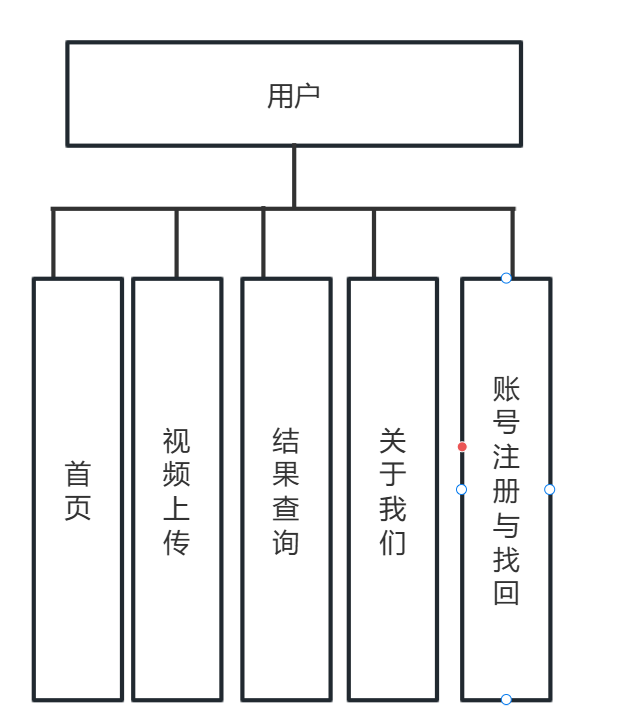
\includegraphics[width=0.3\textwidth]{source/img/user_uml.png}
    \bicaption{用户用例图}{User Use Case Diagram}
    \label{fig:user-uml}
\end{figure}
管理员用户除了一般用户所拥有的功能之外,还添加了数据统计与任务请求导出功能,以方便实验室研究者了解用户真实需求。管理员用户用例图如\ref{fig:admin-uml}所示。
\begin{figure}[ht]
    \centering
    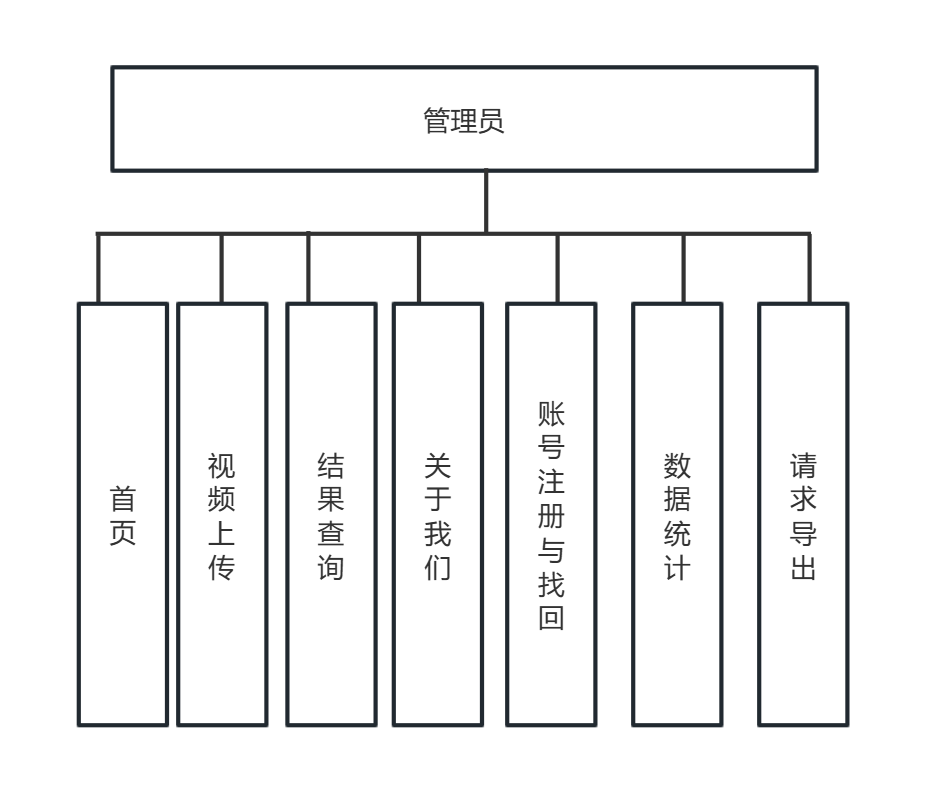
\includegraphics[width=0.4\textwidth]{source/img/admin_uml.png}
    \bicaption{管理员用例图}{Admin Use Case Diagram}
    \label{fig:admin-uml}
\end{figure}

从用例图~\ref{fig:user-uml}和~\ref{fig:admin-uml}分析得出,系统的模块可以划分为:
\begin{itemize}
    \item 首页:作为各个功能模块的入口,完成其他各模块的合理布局;
    \item 用户管理模块:包括用户的注册、登录、注销、密码重置与找回功能;
    \item 任务上传模块:系统的核心功能,完整实现编辑任务上传的全流程;
    \item 结果管理模块:用户在该模块下查询编辑任务的结果,并提供删除、重命名等操作;
    \item 关于我们模块:展示开发者的相关信息;
    \item 数据统计模块:管理员用户在该模块下可以查看用户上传任务的数量、编辑任务的数量、编辑任务的结果数量等数据统计,并导出用户请求数据;
\end{itemize}

\section{模块实现}

本节将介绍系统各个模块的具体实现,包括前端页面、后端接口、数据库设计等。由于首页只作为其余功能模块的载体,
只涉及到前端页面的布局设计,不涉及到与后端的交互;而关于我们模块作为信息展示,仅仅为静态HTML页面,我们也不再详细介绍。
另外,由于各个模块的后端操作都涉及到数据库操作,我们将数据库功能实现单独列出,不再在每个模块中介绍。

\subsection{首页的详细设计与实现}

在前端UI设计中,我们采用Ant Design(Antd)来辅助开发。Antd是一个基于React的UI组件库,提供高质量的React组件,并拥有完整的类型定义文件。

首页的布局采用Antd的Layout组件,使用侧边布局,在左侧放置导航栏以显示各个功能模块,如~\ref{fig:app-dashboard}所示。功能模块间的切换功能通过维护一个全局的
组件状态selectedMenu来实现,导航栏的每一项对应selectedMenu的一个值,检测到用户点击动作时,更新状态为对应的值。

\begin{figure}[ht]
    \centering
    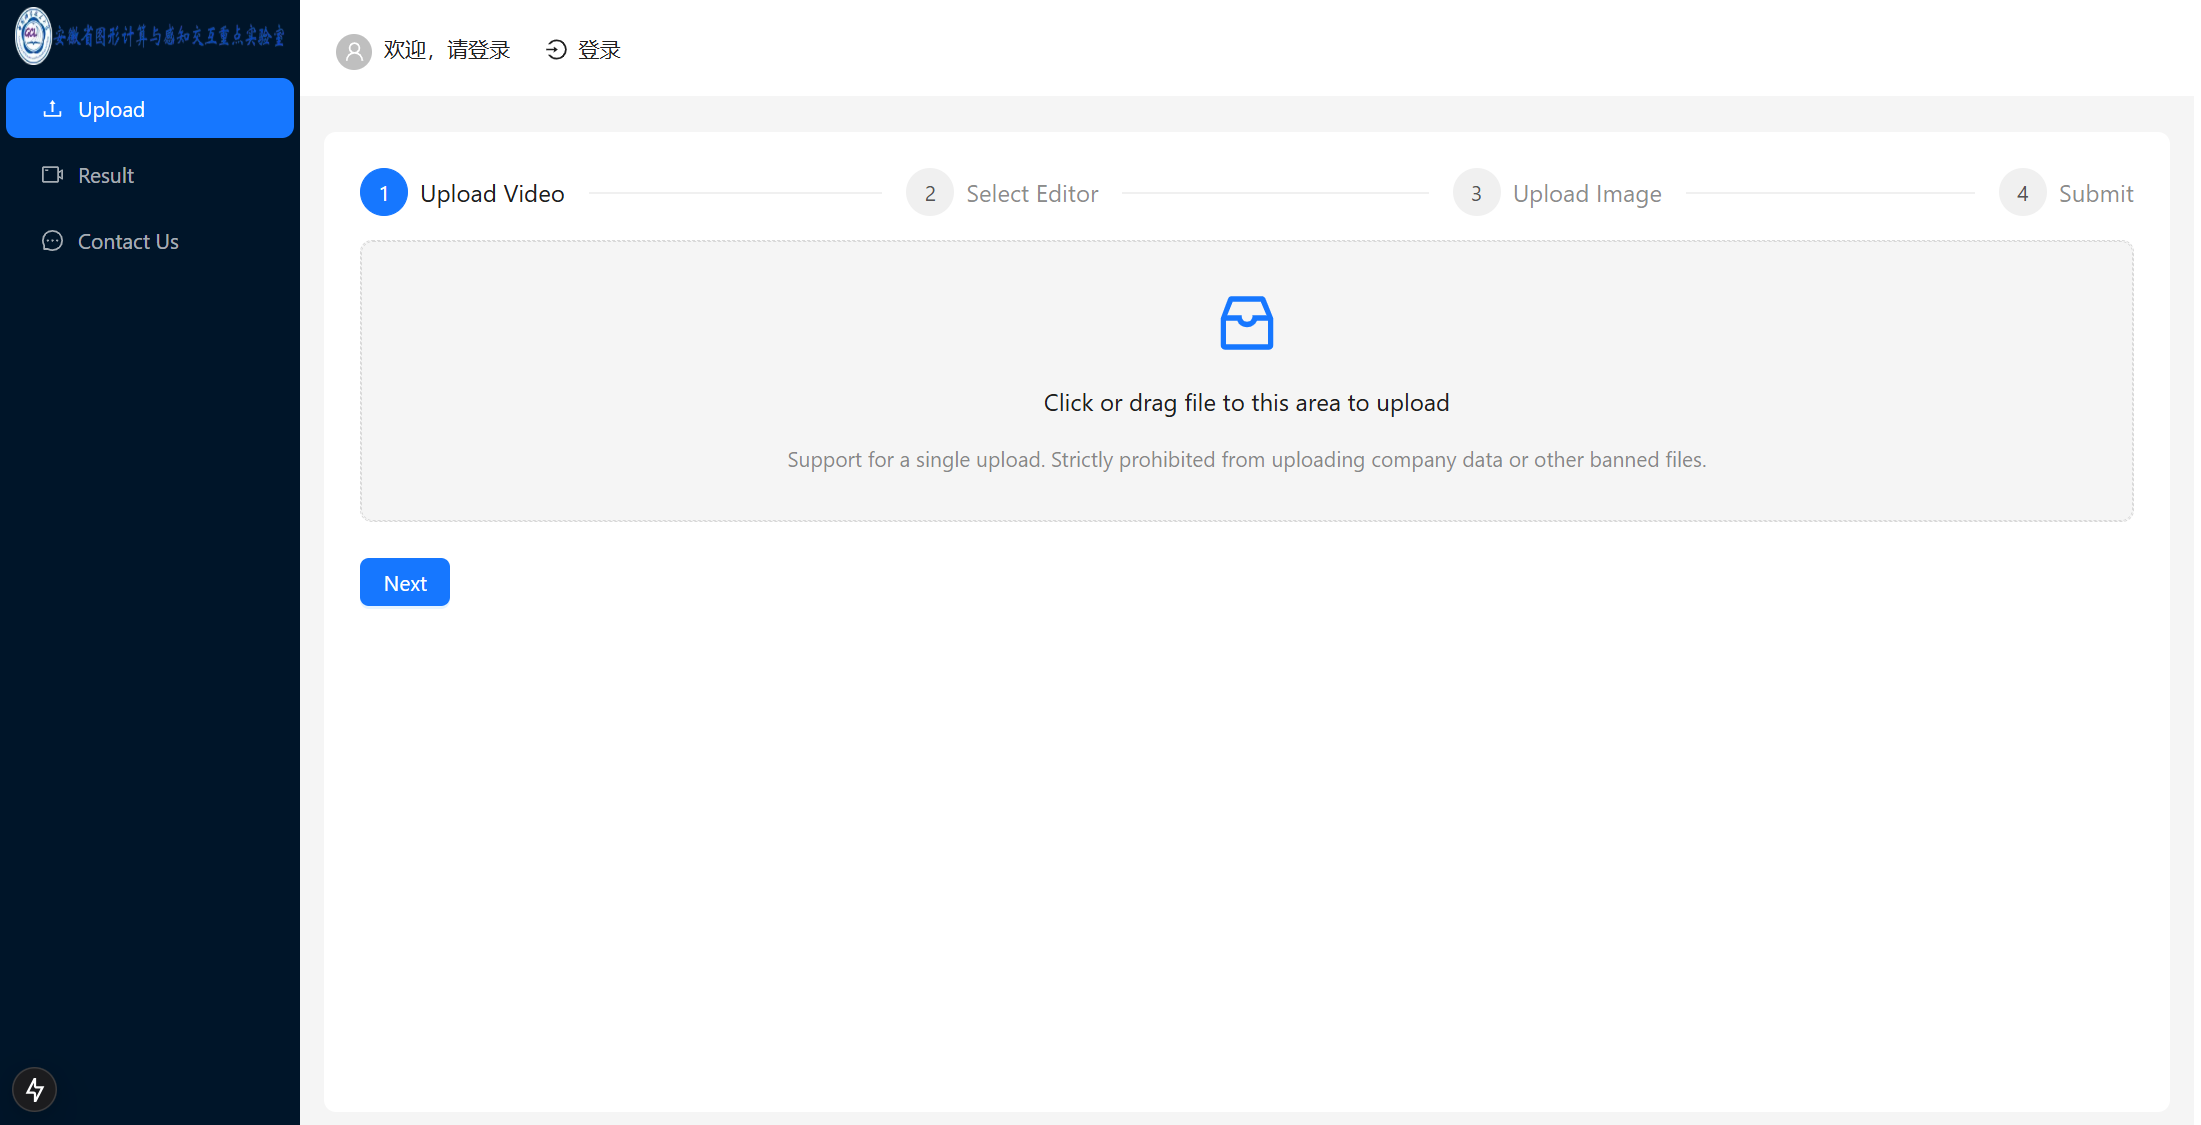
\includegraphics[width=0.8\textwidth]{source/img/app_dashboard.png}
    \bicaption{首页布局}{Home Page Layout}
    \label{fig:app-dashboard}
\end{figure}

为了显示对应模块的内容,我们在Layout组件的Content区域设置条件渲染,根据组件状态selectedMenu的值来渲染不同的组件。
例如selectedMenu的默认值是1,对应任务上传模块,首页默认渲染任务上传组件。此外首页根据用户是否为管理员对导航栏也
进行条件渲染,只有管理员用户才能显示额外的数据统计模块。

\subsection{用户管理的详细设计与实现}

\subsubsection{流程设计}

我们设计的用户登录流程如\ref{fig:login-process}所示,图中包含我们需要实现的三个子流程:用户注册、用户登录与密码找回。
\begin{figure}[ht]
    \centering
    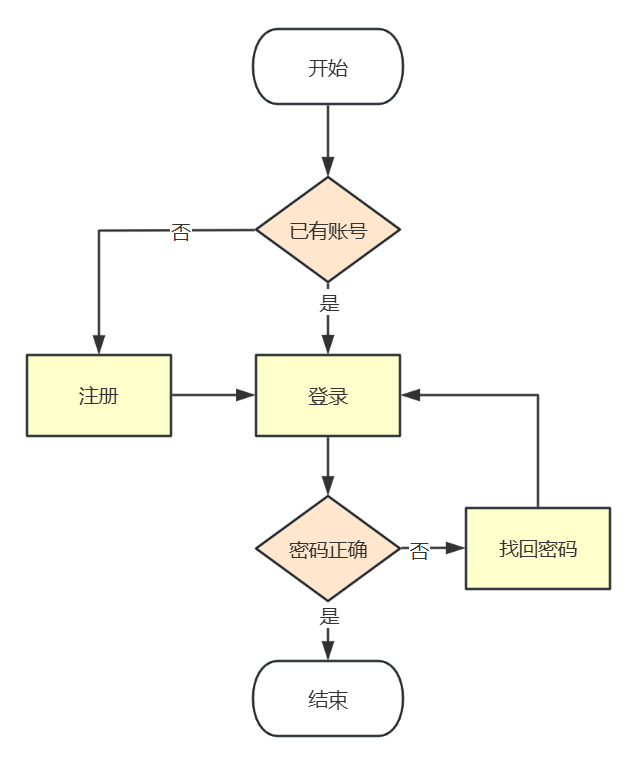
\includegraphics[width=0.4\textwidth]{source/img/login_process.png}
    \bicaption{登录流程图}{Login Process}
    \label{fig:login-process}
\end{figure}

\subsubsection{前端实现}

我们分别为这三个子流程设计了路由页面,并在页面中设置了路由跳转,保证用户页面跳转的双向性。我们使用Antd的Form组件来实现
表单的创建,我们通过设置组件成员的rules属性来设置表单内容检查,包括密码长度、密码复杂度、邮箱是否合法等;
组件中封装的提交按钮通过绑定自定义触发函数以处理提交事件,触发函数的主要逻辑为将后端api需要的数据封装为json格式,
通过axios发送post请求到后端,并处理返回结果。

由于系统中结果查询、上传限制查询等功能都需要使用用户信息,我们又无法频繁地要求用户录入信息,因此在登录流程中,
我们需要维护全局的用户状态以供其他模块使用。为了携带cookies信息到全局,我们选择了使用localStorage来存储用户信息,
在用户登录成功后,我们存储全局的用户信息并设置过期时间,在用户登出时,我们清除全局的用户信息。当其他模块需要使用
用户信息时,只需要从localStorage中解析出所需要的字段即可。

密码找回功能由于涉及到敏感信息,存在安全风险,因此我们设计了两步找回方式。我们需要用户输入邮箱,验证邮箱验证码通过后
自动跳转到密码重置页面,并由后端返回token,用户在重置密码时需要携带token,后端验证token后才能重置密码。这种设计可以防止
用户直接进入重置密码路由对数据库进行攻击,相比于临时生成动态路由,避免了动态路由规则被暴力破解的风险。

\subsubsection{后端实现}

后端主要实现的功能包括验证邮件发送、token生成与验证。

\subsection{任务管理的详细设计与实现}

\subsubsection{任务上传}

根据视频编辑算法的输入,需要用户提供视频、编辑提示类型与对应的提示内容,并提供邮箱以获取编辑结果。上传流程如\ref{fig:upload_process}所示。
\begin{figure}[ht]
    \centering
    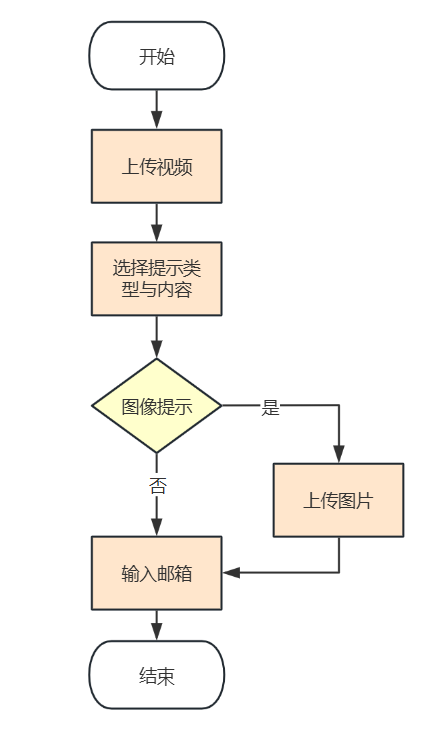
\includegraphics[width=0.3\textwidth]{source/img/edit_process.png}
    \bicaption{上传流程图}{Upload Process}
    \label{fig:upload_process}
\end{figure}

\subsection{结果管理的详细设计与实现}

\subsubsection{结果管理}

用户在结果查询界面可以查看自己上传的任务进度与结果,系统也支持任务重命名与删除,同时在任务处理完成后会自动生成略缩图,方便用户预览结果。

\subsection{数据统计的详细设计与实现}


\subsection{数据库功能实现}

我们使用PyMySQL作为Flask框架下的MySQL数据库驱动,受到SQLAlchemy等ORM驱动框架将数据库操作封装为对象方法的启发,我们
将常用的数据库操作封装为函数,以方便在Flask应用中调用。

我们还在数据库中添加了连接池设计,以提高数据库连接的效率。由于MySQL数据库是通过TCP协议进行通信的,因此每次建立连接都需要进行三次握手,
以实现TCP的可靠传输;而建立TCP连接后数据库还需要传输认证包用于用户验证,因此数据库连接的建立是一个相对耗时的操作。我们采用的连接池设计
通过维护一定数量的数据库连接,在需要时直接从连接池中获取数据库连接,避免了频繁建立数据库连接带来的性能问题。

\subsection{安全控制设计}

在系统构建的过程中,安全控制是一个至关重要的方面。为了防止未经授权的访问和操作,我们需要用户在登录状态下进行操作,这涉及到对用户信息与数据的
加密保护;我们也需要限制用户的操作行为,以防止用户的恶意操作;另外为了保证服务器的安全性,我们也需要系统部署过程中的安全措施。

\subsubsection{用户信息与数据加密}

我们将用户信息存储在数据库中,包括用户名、密码、邮箱等敏感信息。为了保证用户信息的安全性,我们对输入信息加密后存储。
我们使用密钥派生函数(Key Derivation Function, KDF)将用户提供的弱密码根据一些额外参数生成强密码,具体来说,
我们将用户的密码与给定的盐值(salt)连接起来,利用SHA256等加密函数经过多轮迭代得到最终的密码哈希值。由于哈希函数
具有单向性,我们无法通过哈希值反推原始密码,因此在验证用户密码时,我们只能重新计算哈希值并与存储的哈希值进行比较。

这种加密方式通过刻意使密钥派生的速度变慢,从而增加暴力破解的难度;同时由于不同密钥对应的盐值不同,确保了即使相同的密码
也会产生不同的哈希值,能够抵抗彩虹表攻击。

\subsubsection{用户行为限制}

为了防止用户恶意操作,如短时间大量上传文件、大量提交任务等,我们对用户行为做出一定的限制。具体包括:
\begin{itemize}
    \item 用户上传的文件在没有提交任务时被设置为一小时过期,未使用的文件达上限时拒绝用户的上传行为;
    \item 由于任务处理需要一定的时间,我们限制用户在处理的任务数量上限,超过限制则拒绝用户提交任务;
\end{itemize}
这些限制的具体实现通过MySQL数据库的触发器和在后台运行的定时任务完成。在插入数据时过期时间被设置为一小时后,当有任务使用到
对应文件时,UsedByProjectID字段外键引用任务ID;任务被删除时外键引用设置为NULL,触发器检测到后将时间设置为当前时间,文件过期。
后台的定时任务通过查询文件的过期时间字段来定时删除过期的文件。

\subsubsection{部署安全措施}

为了保证服务器的安全性,我们采取了以下措施:
\begin{itemize}
    \item 限制服务器中部署用户组的权限,避免系统文件遭到篡改;
    \item 文件传输使用HTTPS协议传输,通过SSL/TSL协议建立加密的传输通道
    \item 服务器部署在内网,限制外部访问,在网关上设置防火墙。
\end{itemize}
\chapter{测试评估}

在完成系统实现后,我们对系统进行功能与非功能性测试,以验证其是否符合预期,并评估其性能。
本章将详细介绍测试方法、测试结果以及性能评估。

\section{测试环境}

为了确保测试结果的准确性与可靠性,我们采用与实际部署环境相似的硬件和软件配置进行测试,~\ref{tab:hardware-env}与
~\ref{tab:software-env}分别展示了测试环境的硬件和软件配置。

\begin{table}
    \centering
    \bicaption{硬件环境}{Hardware Environment}
    \label{tab:hardware-env}
    \resizebox{0.5\linewidth}{!}{
    \begin{tabular}{cl}
        \toprule
        类型   &  配置信息       \\
        \midrule
        CPU & 2x Intel Xeon Gold(2.90GHz,64核/128线程) \\
        GPU & 8x NVIDIA RTX 4090(24GB显存/卡)\\
        存储架构 & NUMA(2节点)\\
        驱动版本 & CUDA 12.2\\
        \bottomrule
    \end{tabular}
    }
\end{table}

\begin{table}
    \centering
    \bicaption{软件环境}{Software Environment}
    \label{tab:software-env}
    \resizebox{0.5\linewidth}{!}{
    \begin{tabular}{cl}
        \toprule
        类型   &  配置信息       \\
        \midrule
        Next.js & 15.1.2 \\
        node.js & 22.14.0 \\
        Python & 3.9.21 \\
        flask & 3.1.0 \\
        客户端 & Google Chrome 135.0.7049.115 \\
        \bottomrule
    \end{tabular}
    }
\end{table}


\include{chapters/floats}
\include{chapters/math}
\include{chapters/citations}

\chapter{结论}

\bibliography{bib/ustc}  % 参考文献使用 BibTeX 编译
% \printbibliography       % 参考文献使用 BibLaTeX 编译

\appendix
% !TeX root = ../main.tex

\chapter{补充材料}


\section{系统运行展示}

为了更直观地说明系统的运行情况,我们在这里通过运行截图辅以文字说明的方式来进行展示。

\subsection{用户管理展示}

进入系统后自动跳转至dashboard路由,对应系统的主面板,如\ref{append:dashboard}所示。

\begin{figure}[ht]
    \centering
    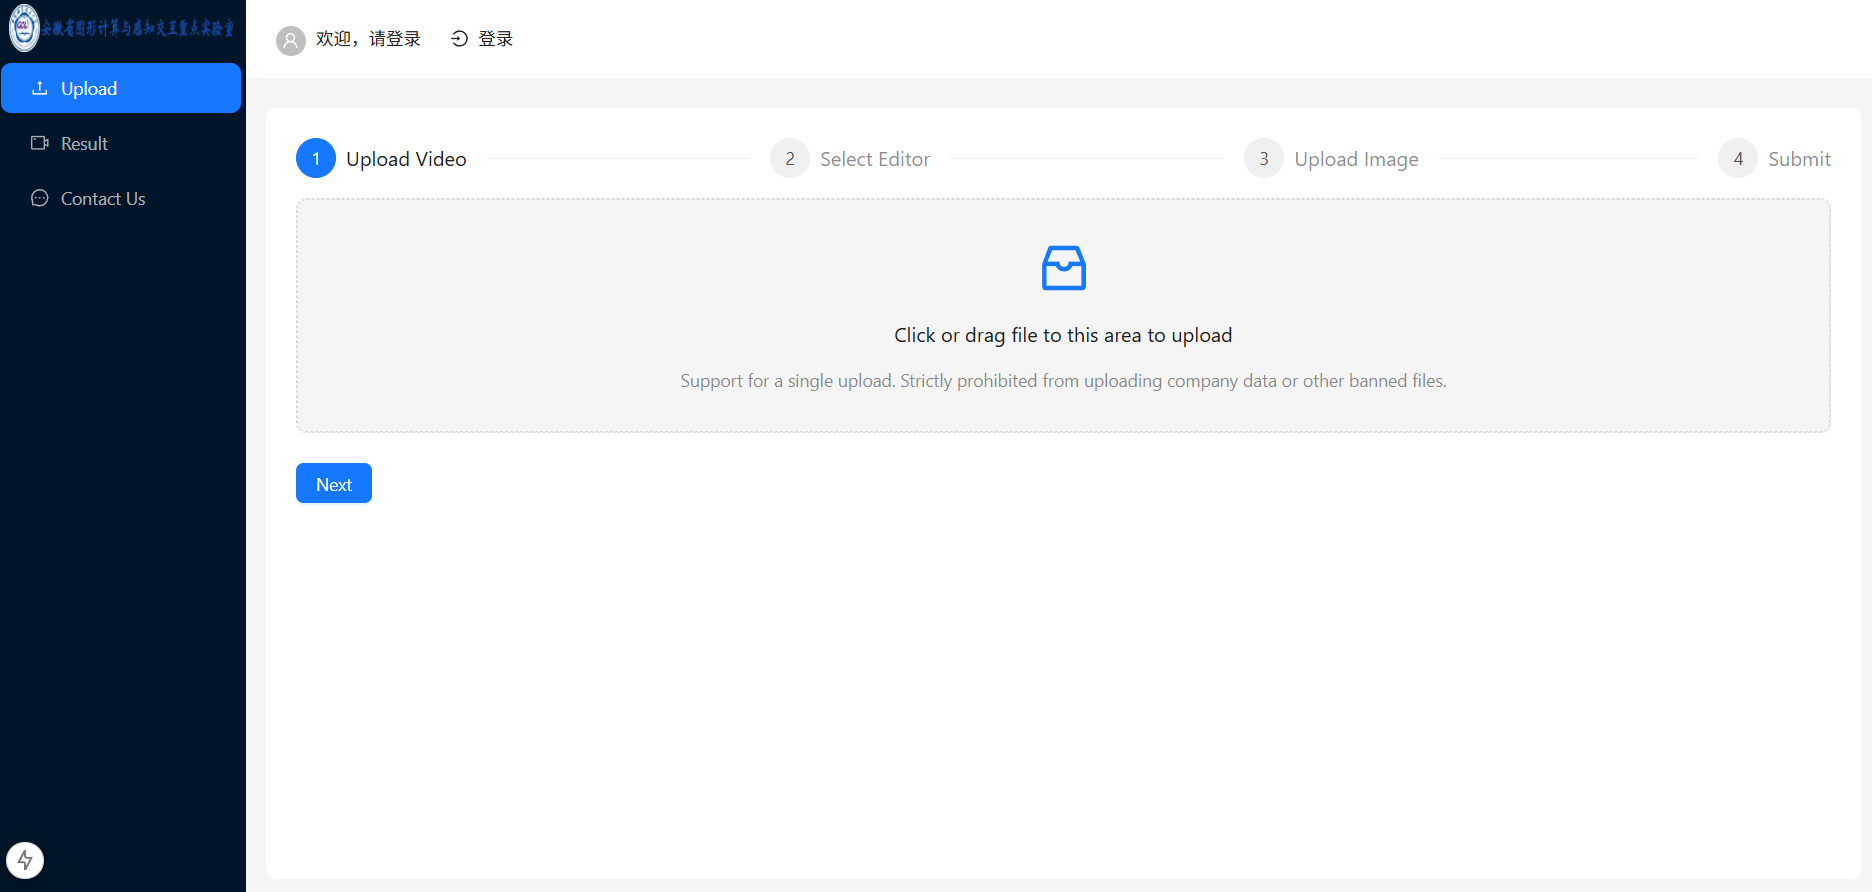
\includegraphics[width=0.8\textwidth]{source/append/dashboard.png}
    \caption{系统主界面}
    \label{append:dashboard}
\end{figure}


\backmatter
% !TeX root = ../main.tex

\begin{acknowledgements}

站在春日的尾声回望,庭梧新绿初展,叶叶如掌。值此论文付梓之际,才惊觉四年时光竟如春樱般翩然将逝。

首先,感谢我的父母。二十余载春秋,我在你们无私的爱中长大。漫漫求学路上,你们一直给予我包容与支持,让我能够走自己想走的路,
追求自己的梦想。成为你们的孩子,是我此生最大的幸运。

感谢我的导师张举勇教授。您严谨的治学态度与睿智的学术见解,如明灯般照亮我学术探索的每一步。无论是在我的保研、留学申请,
还是在我的毕业论文撰写过程中,您都给予了我细心的指导与宝贵的帮助。您的教诲将伴随我一生,成为我不断前行的动力。

感谢实验室的郭玉东特任副研究员,高玄学长与杨圣铭学长。在我的研究遇到瓶颈时,你们给予了我无私的帮助与指导,让我能够顺利完成论文的关键部分。

感谢我的母校中国科学技术大学和数学科学学院。四年前,我怀揣着对数学的热爱和对科学的向往,踏入了这片沃土。四年的时光,我如愿学习到了
渴望的知识,结识了志同道合的朋友,也收获了宝贵的经历。即便四年后的今天我已不再坚持当年数学理论研究的梦想,我仍然不后悔来到科大数院的选择。

最后感谢这一年来陪伴在我身边的雨睿同学。琴瑟易鼓,子期难再。能在人海中与你相遇,是岁月予我最好的馈赠。

停笔之时,窗外蝉鸣渐起,方觉已然入夏。

\end{acknowledgements}

\include{chapters/achievements}

\end{document}
